\subsection{Diseño de Zonas de Depósito}

Las zonas de depósito constituyen los receptáculos donde el manipulador deposita los objetos clasificados. El diseño de estos componentes evolucionó a través de un proceso iterativo que permitió identificar y resolver múltiples deficiencias del concepto inicial.

\subsubsection{Primera Iteración: Canecas con Sistema de Imanes}

El diseño inicial contemplaba dos tipos de canecas de diferentes tamaños (Figura \ref{fig:canecasIman}): canecas grandes para objetos voluminosos y canecas pequeñas para objetos de menor tamaño. Ambos tipos incorporaban imanes de neodimio en su base para acoplarse a los módulos cuadrados y rectangulares de la primera iteración de la plataforma base.

\begin{figure}[H]
    \centering
    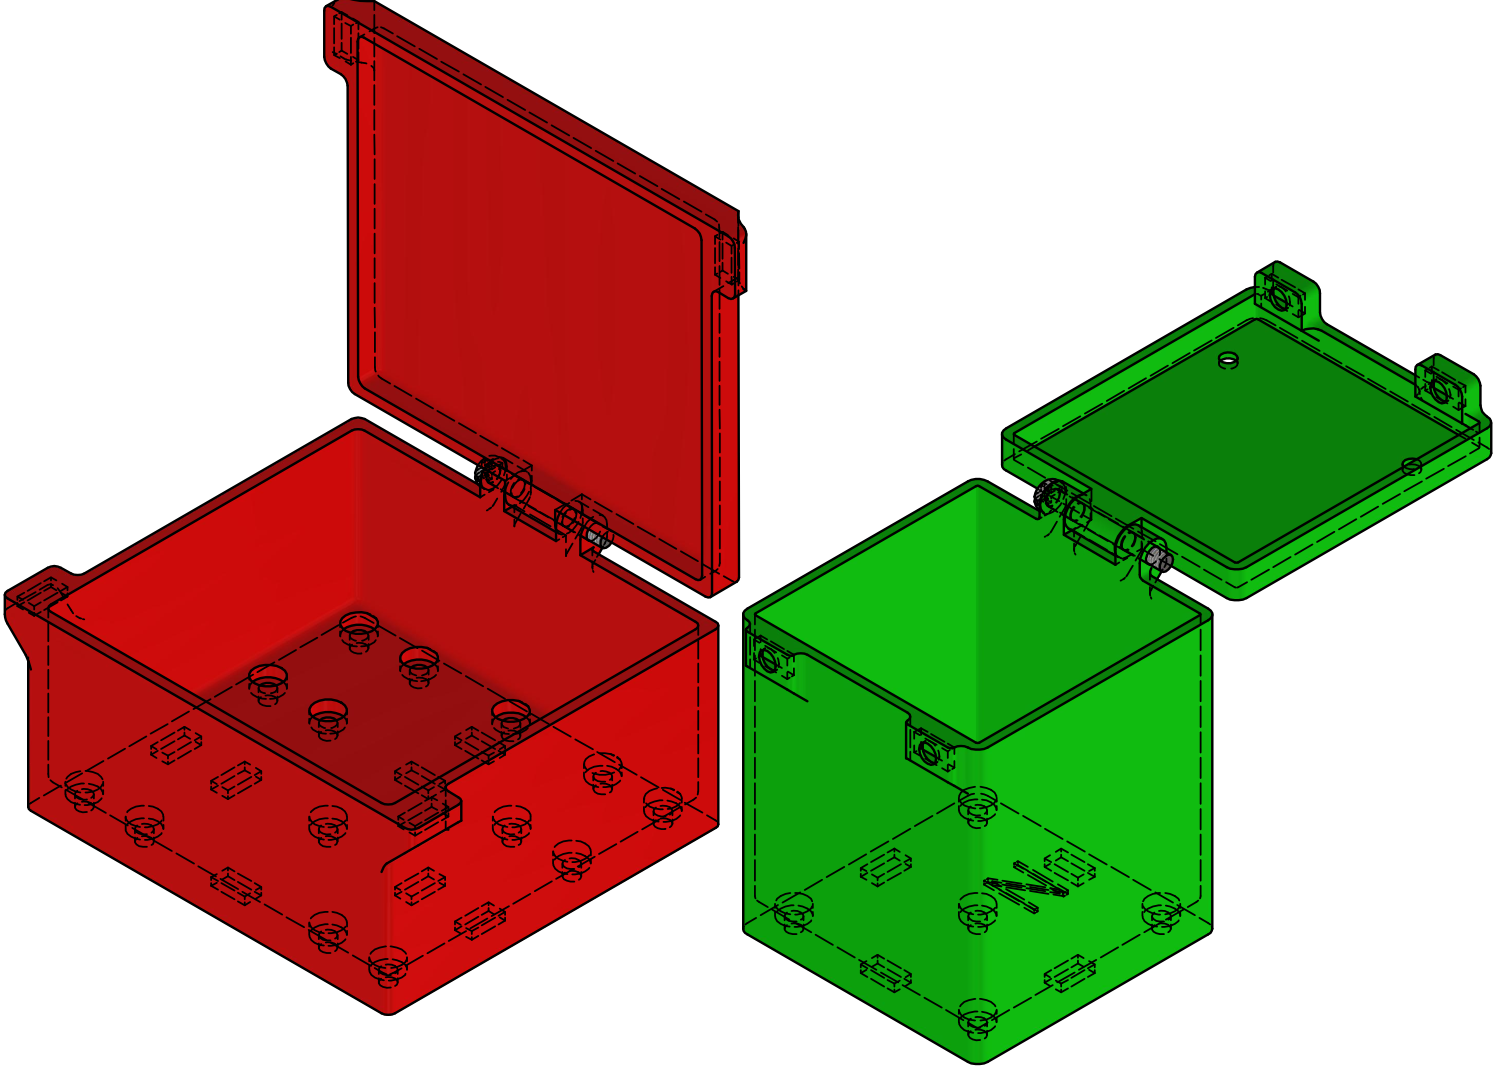
\includegraphics[width=0.7\textwidth]{06disenoConceptual/img/canecas/canecasIman.png}
    \caption{Primera iteración del diseño de zonas de depósito. Se muestran dos tipos de canecas (grande en rojo y pequeña en verde) equipadas con imanes de neodimio en su base y tapas abatibles por bisagra. Ambos diseños incluyen cavidades para alojar imanes y agujeros roscados para fijación opcional a la plataforma.}
    \label{fig:canecasIman}
\end{figure}

Estas canecas incluían tapas con bisagra y agujeros para anclaje permanente opcional a la plataforma. Sin embargo, este diseño fue descartado completamente debido a las siguientes deficiencias críticas:

\begin{enumerate}
    \item \textbf{Dependencia de imanes}: El sistema de fijación basado en atracción magnética resultó insuficientemente robusto para garantizar estabilidad durante las operaciones de depósito y transporte
    
    \item \textbf{Interferencia visual}: Los agujeros de tornillería visibles en la superficie superior comprometían los algoritmos de visión por computador, dificultando la discriminación entre objetos de interés y elementos estructurales (cabezas de tornillos)
    
    \item \textbf{Restricción de accesibilidad}: Las dimensiones de apertura no permitían la entrada de la garra del robot, limitando la funcionalidad exclusivamente a depósito y eliminando la posibilidad de recolección desde las canecas
    
    \item \textbf{Complejidad innecesaria}: El diseño requería múltiples tipos de elementos de fijación (tornillos, tuercas, imanes) aumentando costo y dificultad de ensamblaje
    
    \item \textbf{Aprovechamiento ineficiente del espacio}: El mecanismo de cierre por bisagra generaba volumen muerto en la parte superior de las canecas
\end{enumerate}

\subsubsection{Especificación de Requerimientos para el Rediseño}

A partir de las deficiencias identificadas, se establecieron los siguientes requerimientos para las iteraciones subsecuentes:

\begin{itemize}
    \item La garra del PhantomX Pincher debe poder acceder al interior de las canecas, tanto para depósito como para eventual recolección de objetos
    \item Geometría simple sin artefactos visuales que puedan interferir con los algoritmos de visión por computador
    \item Reducción del número de componentes y simplificación del ensamblaje
    \item Estandarización en un único tipo de caneca para todas las zonas de depósito
    \item Sistema de fijación permanente a la plataforma base
    \item Conservación de sistema de cierre para contención de objetos durante transporte
\end{itemize}

\subsubsection{Análisis Dimensional para Accesibilidad de Garras}

El dimensionamiento de las canecas consideró la compatibilidad con dos variantes del robot PhantomX Pincher disponibles en el laboratorio:

\paragraph{PhantomX Pincher AX-12}
La garra de esta variante (Figura \ref{fig:garraPXP-AX12}) presenta dimensiones de aproximadamente 72 mm de ancho por 61 mm de alto.

\begin{figure}[H]
    \centering
    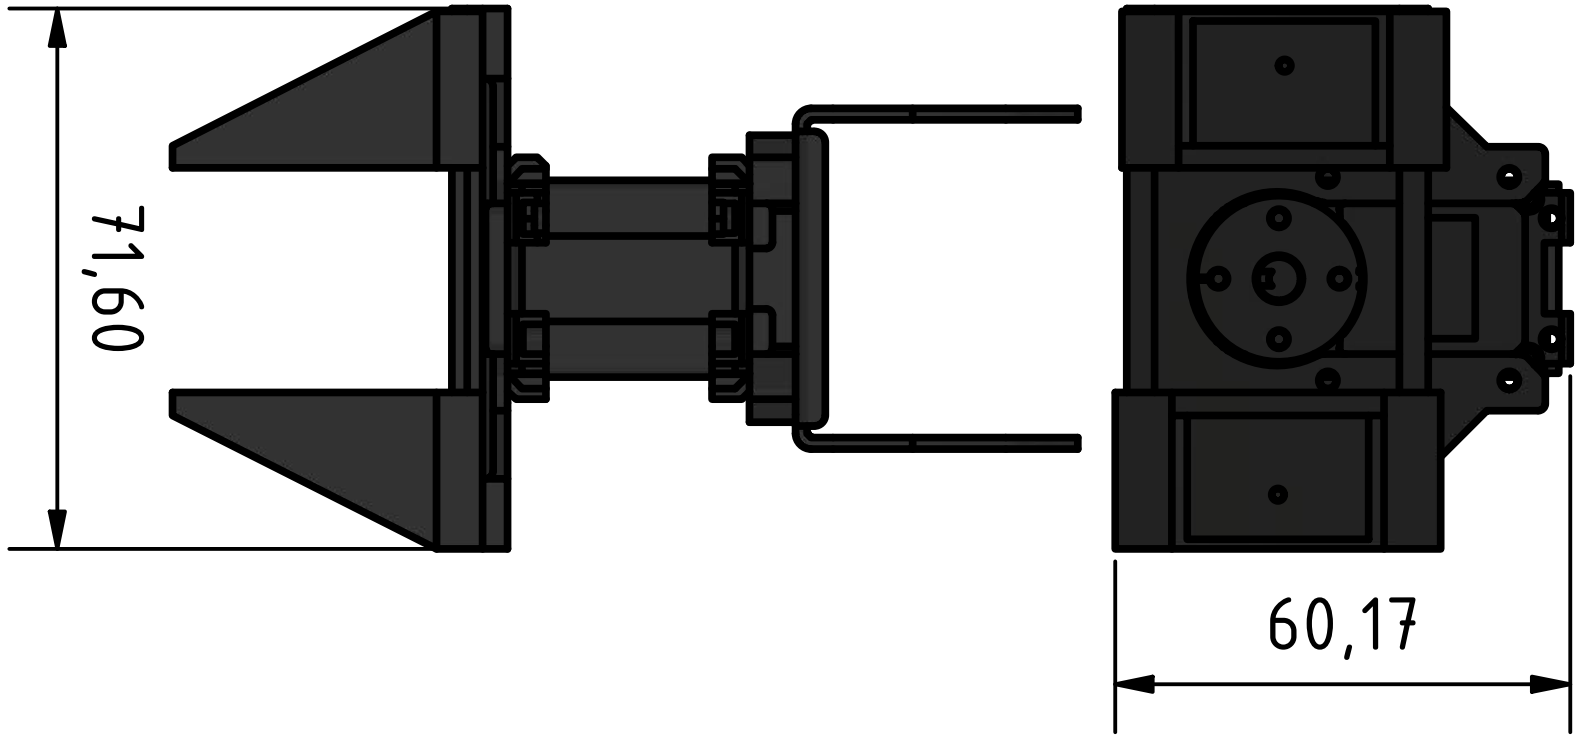
\includegraphics[width=0.5\textwidth]{06disenoConceptual/img/canecas/garraPXP-AX12.png}
    \caption{Garra del robot PhantomX Pincher AX-12. Dimensiones: 72 mm de ancho × 61 mm de alto. Se observan los dedos de la garra (cian) y el servomotor Dynamixel AX-12A (rosa) que controla la apertura/cierre.}
    \label{fig:garraPXP-AX12}
\end{figure}

\paragraph{PhantomX Pincher A100}
La garra de esta variante (Figura \ref{fig:garraPXA100}) posee dimensiones mayores: 104 mm de ancho por 54 mm de alto aproximadamente.

\begin{figure}[H]
    \centering
    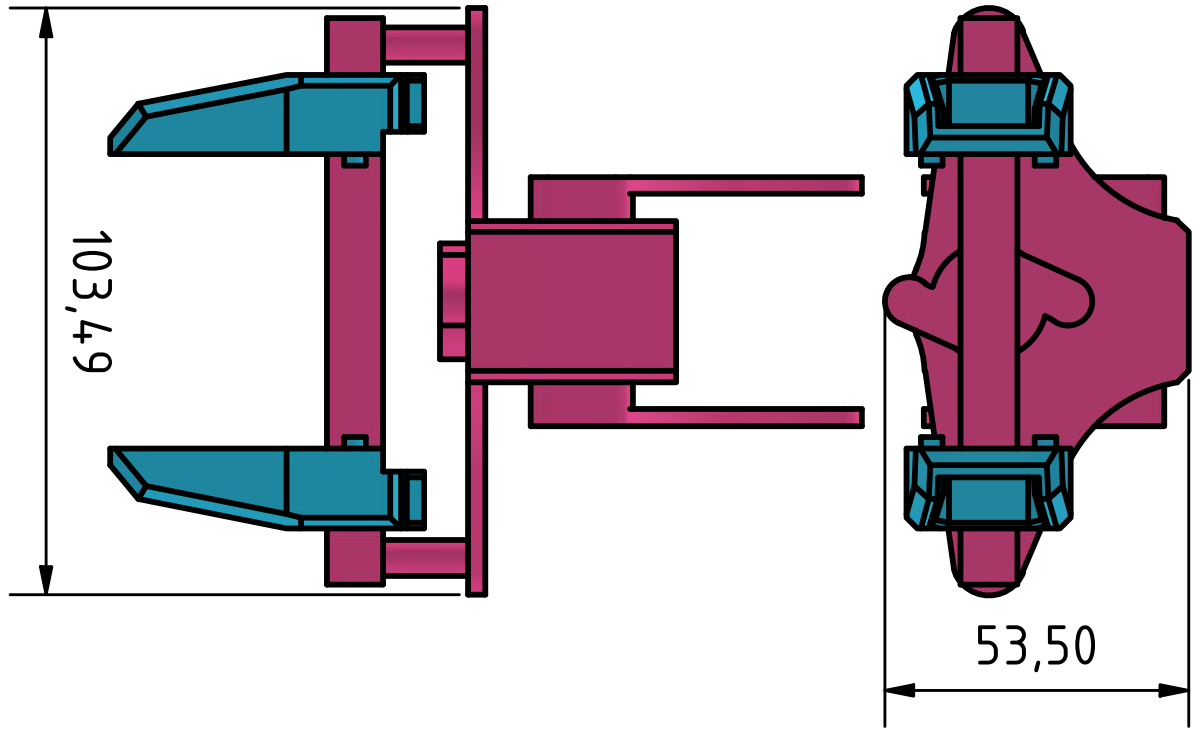
\includegraphics[width=0.5\textwidth]{06disenoConceptual/img/canecas/garraPXA100.png}
    \caption{Garra del robot PhantomX Pincher A100. Dimensiones: 104 mm de ancho × 54 mm de alto. Esta variante presenta mayor apertura máxima que el modelo AX-12.}
    \label{fig:garraPXA100}
\end{figure}

\subsubsection{Diseño Final de las Canecas}

El diseño definitivo de las canecas se desarrolló considerando las restricciones cinemáticas, espaciales y de manufactura identificadas durante el proceso de diseño de la plataforma.

\paragraph{Dimensionamiento Longitudinal}

El largo de las canecas se determinó a partir del ángulo de rotación de 58.9° de las zonas de depósito visible en los layouts de las Figuras \ref{fig:layout1} y \ref{fig:layout2}. Partiendo de este ángulo, se maximizó la dimensión longitudinal sin invadir áreas asignadas a otros componentes, resultando en un ancho exterior de 148 mm y un ancho interior útil de 142 mm.

\paragraph{Apertura Frontal}

Se incorporó una apertura frontal de 131 mm de ancho que permite el acceso de la garra por el frente de la caneca. Esta dimensión proporciona holguras laterales de:
\begin{itemize}
    \item 29 mm por lado para la garra AX-12 (ancho 72 mm)
    \item 13 mm por lado para la garra A100 (ancho 104 mm)
\end{itemize}

Estas holguras son suficientes para permitir el ingreso de las garras considerando tolerancias de posicionamiento del manipulador.

\paragraph{Sistema de Tapa Deslizante}

En la parte inferior de la apertura frontal se incorporó un chaflán de 45° que define una guía para una tapa deslizante. Este diseño ofrece ventajas significativas sobre el sistema de bisagra del diseño anterior:

\begin{itemize}
    \item La tapa no puede ser desplazada verticalmente, permaneciendo cautiva durante el transporte
    \item El movimiento únicamente horizontal facilita las operaciones de cierre
    \item Se elimina el volumen muerto superior presente en el diseño con bisagra
\end{itemize}

\begin{figure}[H]
    \centering
    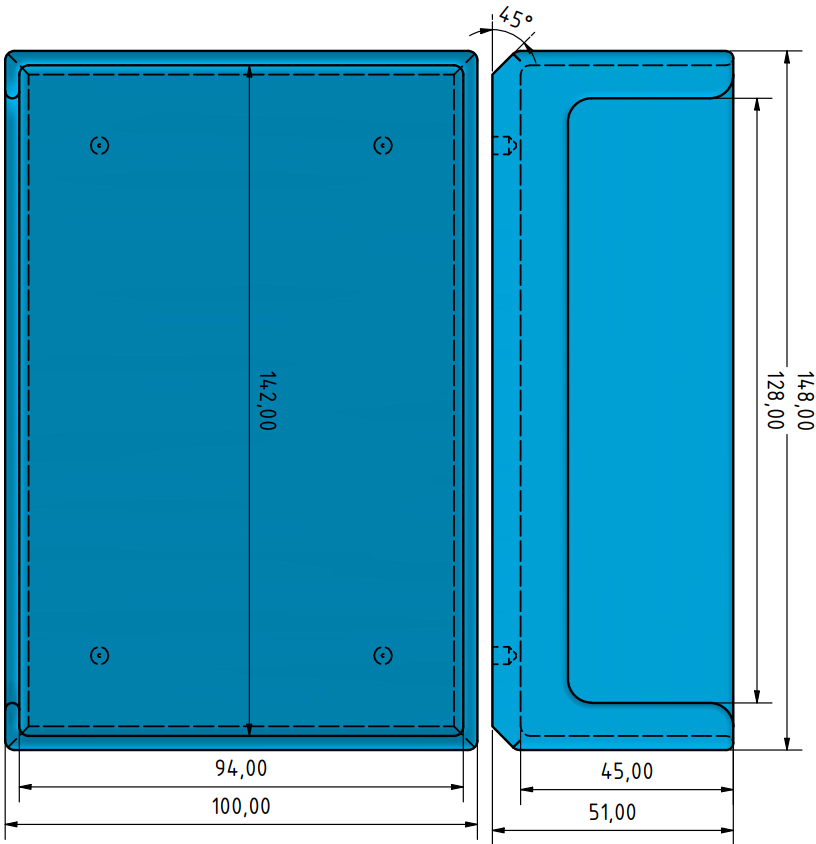
\includegraphics[width=0.8\textwidth]{06disenoConceptual/img/canecas/canecaMedidas.png}
    \caption{Vistas ortogonales de la caneca final con dimensiones principales. Vista superior: 100 mm × 94 mm exteriores, interior de 142 mm de profundidad. Vista lateral: altura total de 148 mm (128 mm útiles), profundidad de 51 mm (45 mm útiles). Se observa el chaflán de 45° para la guía de la tapa deslizante y las posiciones de los insertos roscados M3.}
    \label{fig:canecaMedidas}
\end{figure}

\paragraph{Sistema de Fijación con Insertos Térmicos}

Se implementó un sistema de fijación mediante cuatro insertos roscados M3 para plástico ubicados en la base de la caneca. Estos insertos se instalan mediante inserción térmica: se calientan y se introducen en cavidades cilíndricas diseñadas específicamente, donde el plástico circundante se funde parcialmente y fluye hacia las ranuras del inserto, creando una unión mecánica permanente al enfriarse.

Este sistema ofrece múltiples ventajas:
\begin{itemize}
    \item Los tornillos M3 que fijan la caneca a la plataforma quedan ocultos en la cara inferior, eliminando elementos visuales en la superficie superior
    \item Las roscas metálicas resisten ciclos repetidos de montaje/desmontaje sin degradación
    \item No se requieren tuercas, simplificando el ensamblaje
    \item La superficie superior de la caneca queda completamente limpia, optimizando el desempeño de los algoritmos de visión por computador
\end{itemize}

\paragraph{Separadores de Altura}

Se incorporaron cuatro separadores entre la plataforma base y la caneca. Estos separadores cumplen dos funciones esenciales:

\begin{enumerate}
    \item Nivelar la altura de las canecas con la zona de recolección, que es una pieza elevada respecto a la plataforma base
    \item Proporcionar el espacio necesario para que la tapa deslizante pueda desplazarse completamente y cerrar la caneca
\end{enumerate}

\paragraph{Ensamble Completo}

El subconjunto completo de la zona de depósito se presenta en la Figura \ref{fig:ensambleCanecaTapaSlide}.

\begin{figure}[H]
    \centering
    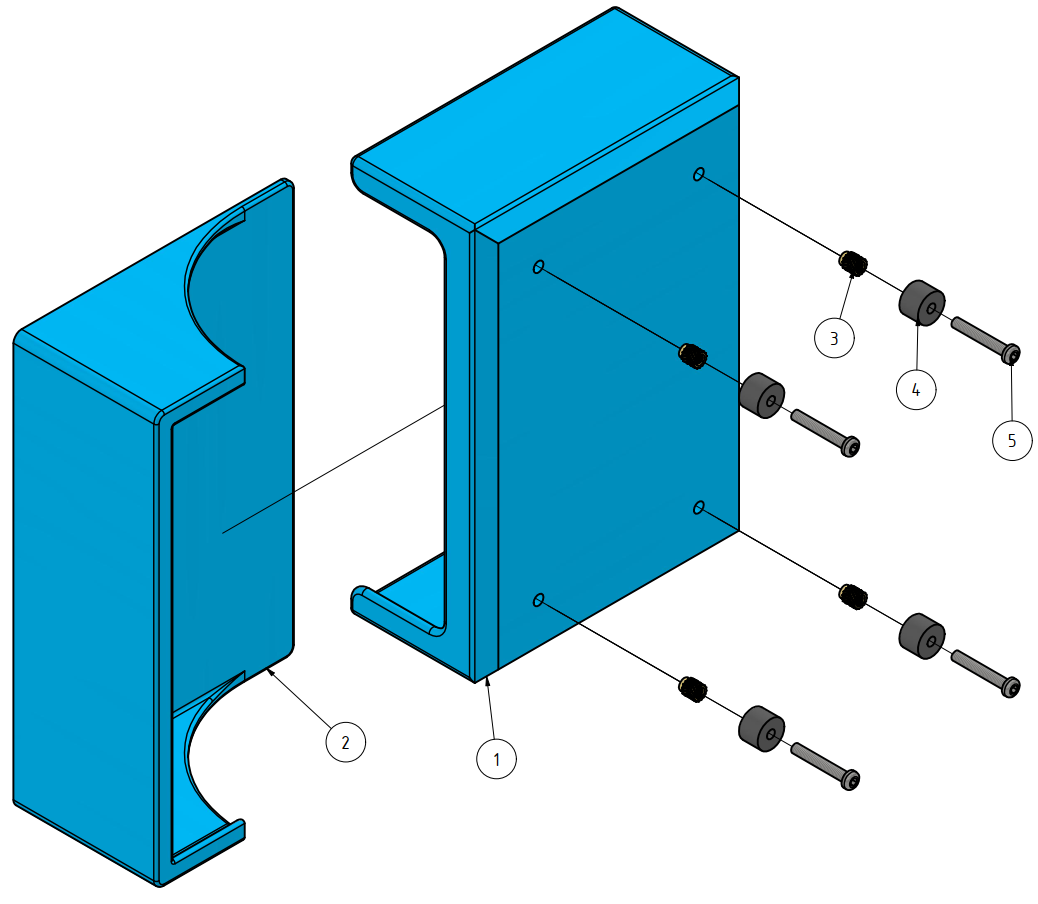
\includegraphics[width=0.8\textwidth]{06disenoConceptual/img/canecas/ensambleCanecaTapaSlide.png}
    \caption{Ensamble explosionado del conjunto de zona de depósito. (1) Cuerpo de la caneca fabricado mediante FDM, (2) Tapa deslizante, (3) Insertos roscados M3 de latón para instalación térmica, (4) Separadores de altura, (5) Tornillos M3 × 20 mm que atraviesan separadores y caneca para fijarse en insertos roscados de la plataforma base.}
    \label{fig:ensambleCanecaTapaSlide}
\end{figure}

\begin{table}[H]
\centering
\caption{Lista de materiales del conjunto de zona de depósito}
\label{tab:bom_caneca}
\small
\begin{tabular}{|c|l|c|l|l|}
\hline
\textbf{\#} & \textbf{Componente} & \textbf{Cant.} & \textbf{Fabricación} & \textbf{Material} \\
\hline
1 & Caneca & 1 & FDM & PLA/ABS \\
2 & Tapa deslizante & 1 & FDM & PLA/ABS \\
3 & Inserto roscado M3 & 4 & Comercial & Latón \\
4 & Separador & 4 & FDM & PLA/ABS \\
5 & Tornillo M3 × 20 mm & 4 & Comercial & Acero \\
\hline
\end{tabular}
\end{table}

El diseño final de las zonas de depósito representa una solución optimizada que equilibra accesibilidad robótica, simplicidad de manufactura, robustez mecánica y compatibilidad con sistemas de visión por computador, resolviendo todas las deficiencias identificadas en la iteración inicial.